\documentclass{report}
\usepackage{graphicx}
\usepackage{float}

\graphicspath{{./images/}}

\floatstyle{boxed}
\restylefloat{figure}

\begin{document}

\tableofcontents
\listoffigures

\chapter{Introduction}

Introduction

\chapter{Functional Requirements}

\section{High-level functionality}
The high level functionality of this system can be broken down into several
major sections. Sensors play a major role in interfacing the real world with
the several other sections of the controller. Physical security, both inside
and outside of the home is important. This goes hand in hand with family
security once family members have left the premises of the household. Finally,
green energy management can be easily integrated with the other systems to
ensure prudent usage of resources. 

\subsection{Sensors}
% TODO :: proof read this. It may not all make sense

% TODO :: elaborate HVAC or put it in the glossary
The most crucial part of the system that ties all of the other parts together
is the sensor network. They are the interface between the real world and the
controllers. They detect if the house has been intruded upon by outsiders
through sensors on the windows and doors. They can alert the family if somebody
left the stove top on. Living patterns can be established and monitored to
warn of health problems or to control the HVAC so that energy is not wasted
when nobody is home or they are all asleep. Cameras, motion detectors, hall
effect sensors, and other miscellaneous sensors comprise the majority of this
network.

Cameras play multiple roles in the sensor network. Facial recognition can be
used to detect family members entering and leaving the house to track their
activities. They can be used to alert when strangers are approaching the door
or are on the premises in either a friendly manner or in a more cautious one
depending on the family members currently at home.

Motion detectors provide the security system with the means to trigger alerts 
when motion is detected in certain areas of the home while the system is armed. 
A network of motion detector sensors will be positioned in the hallways of the home, 
with particular attention to entries to the home. Motion detectors outside the 
house will be able to control the lighting system such that people approaching the 
home can be illuminated and easily identified.

Temperature sensors and hall effect sensors are two other major components.
Temperature sensors can be used by both physical security, to ensure that the
oven has not been on for an extended period of time without user interaction as
well as for green energy management to control the overall temperature of the
house or each room. Hall effect sensors can be used with temperature sensors to
detect if windows or doors have been left open when they should be closed in
order to prevent wasting energy. These sensors can also be used to detect
intruders attempting to break in through windows or doors.

\subsection{Family Safety}

In addition to necessary home security functionality, the system will incorporate 
methods to provide safety to members of the users' family. Child safety is a particular 
concern that will be addressed by this portion of the home security system. Sensors 
will be implemented on cabinets as well as certain areas of the home that may contain 
hazardous materials that could be harmful to children. Contact sensors will be present 
on medicine cabinets, closets with cleaning materials, and knife drawers to alert the user
that these areas of the home have been accessed.

\subsection{Security System}

\subsection{Green Energy Management}



\section{Scenarios}

\subsection*{Arming the System - NFC Device}

The resident is leaving the home and wishes to arm the security system. The resident can
do so by approaching the security console and holding their NFC device within 0.2 meters
of the interface. The resident must hold their NFC device near the console until the device
is read and identified by the system as belonging to the resident of the home. Once this is
confirmed, the user may leave the home while the system initiates the arm countdown. Once
the system completes the countdown, the system has been successfully armed.

\subsection*{Disarming the System - NFC Device}

The procedure for disarming the system using an NFC device is very similar to the arming
procedure. The resident enters the home at which point the disarm countdown begins. The
resident holds his NFC device up to the console to disarm the system. The NFC device is
identified and the security system is disarmed and the countdown is interrupted.

\subsection*{Arming the System - Keypad}

The resident wishes to arm the security system, but is not in possession of an NFC device.
The resident can arm the system by entering a valid security code. Once the code has been
entered, it is validated by the system. The system initiates the arm countdown, and the
resident may now leave the home. The arm countdown completes and the system is now armed.

\subsection*{Disarming the System - Keypad}

The procedure for disarming the system using the keypad is very similar to the arming
procedure. The resident enters the home at which point the disarm countdown begins. The
resident enters a valid security code into the console using the keypad to disarm the system. 
The NFC device is identified and the security system is disarmed and the countdown is interrupted.

\subsection*{Window Intrusion}
%TODO what happens during the alarm state?

The security system is in the armed state. An intruder attempts to open a window from outside
the home. The system receives a signal from the window's sensor that notifies the system that
a window has been opened. The system enters its alarm state.

\subsection*{Door Intrusion}
%TODO what happens during the alarm state?

The security system is in the armed state. An intruder picks the lock on the front door and opens it.
The system begins the alarm countdown alongside audible beeping once the intruder opens the door.
The intruder leaves the premises while the countdown continues. The countdown reaches zero and the
system enters the alarm state.

\subsection*{Fridge Left Open}

The resident opens the fridge door for a drink, and does not close it fully. Unaware, the resident leaves
the kitchen and sits down in the living room. Meanwhile, a countdown has begun while the fridge door
remains open. The countdown finishes and a notification is sent to the resident via SMS. The kitchen speaker
broadcasts an audible message stating that the fridge door has been left open. The user enters the
kitchen and closes the fridge door, resetting the system. 

\subsection*{Childproof Cabinets}

A child in the home has accessed a cabinet that contains hazardous or dangerous materials. The
contact sensor installed on the cabinet door triggers a countdown. When the countdown reaches
zero, and audible alarm is produced and an SMS is sent to the resident of the home to notify them
of the event.

Separately, an adult resident of the home accesses the same cabinet. The contact sensor on the
cabinet door triggers the countdown. The resident pushes a hidden actuator located on the
inside of the cabinet to halt the countdown. The resident closes the cabinet door when he / she is
finished and the sensor notifies the process to go back to its normal wait state.

\subsection*{Child Bedroom Safety}
% TODO how does the resident arm the child safety system? With their phone? Console in the bedroom? 

The resident of the home has placed his child in the crib for the night. When the resident leaves
the bedroom, he arms the child bedroom safety system and closes the door. During the middle
of the night, the child climbs out the crib and falls to the floor. Motion sensors installed in the room
detect this unexpected activity and sound an alarm in the parents' bedroom to notify them of the
event.

\section{Use case model}

\begin{tabular}{| l | p{7cm} |}
\hline
Use case name & \texttt{NFCDisarmSystem} \\ \hline
Participating Actors & Initiated by \texttt{Resident} \\ \hline
Flow of Events & 

\begin{enumerate}
 \item The \texttt{Resident} enters the home while in possession of an NFC device.
 \item The system begins the disarm countdown.
 \item The \texttt{Resident} approaches the console and holds the NFC within 0.2 meters of the console.
 \item The data on the NFC device is read and validated by the system.
 \item The system enters the disarmed state and the disarm countdown is halted.
\end{enumerate}

\\ \hline

Entry Condition & The system is in the armed state and the Resident
enters the home in possession an NFC device. \\ \hline

Exit Condition & The system is disarmed. \\ \hline
Quality requirements & TODO \\ \hline

\hline
\end{tabular}

\begin{tabular}{| l | p{7cm} |}
\hline
Use case name & \texttt{KeyPadDisarmSystem} \\ \hline
Participating Actors & Initiated by \texttt{Resident} \\ \hline
Flow of Events & 

\begin{enumerate}
 \item The \texttt{Resident} enters the home.
 \item The system begins the disarm countdown.
 \item The \texttt{Resident} approaches the console and enters their code using the keypad on the console.
 \item The entered code is validated by the system.
 \item The system enters the disarmed state and the disarm countdown is halted.
\end{enumerate}

\\ \hline

Entry Condition & The system is in the armed state and the Resident
enters the home. \\ \hline

Exit Condition & The system is disarmed. \\ \hline
Quality requirements & TODO \\ \hline

\hline
\end{tabular}

\begin{tabular}{| l | p{7cm} |}
\hline
Use case name & \texttt{NFCArmSystem} \\ \hline
Participating Actors & Initiated by \texttt{Resident} \\ \hline
Flow of Events & 

\begin{enumerate}
 \item The \texttt{Resident} approaches the console and holds the NFC within 0.2 meters of the console.
 \item The data on the NFC device is read and validated by the system.
 \item The system begins the arm countdown.
 \item The \texttt{Resident} leaves the home.
 \item The system arm countdown completes and the system enters the armed state.
\end{enumerate}

\\ \hline

Entry Condition & The system is in the disarmed state and the \texttt{Resident} wishes to arm it 
using an NFC device. \\ \hline

Exit Condition & The system is armed. \\ \hline
Quality requirements & TODO \\ \hline

\hline
\end{tabular}

\begin{tabular}{| l | p{7cm} |}
\hline
Use case name & \texttt{KeyPadArmSystem} \\ \hline
Participating Actors & Initiated by \texttt{Resident} \\ \hline
Flow of Events & 

\begin{enumerate}
 \item The \texttt{Resident} approaches the console and enters their code.
 \item The entered code is validated by the system.
 \item The system begins the arm countdown.
 \item The \texttt{Resident} leaves the home.
 \item The system arm countdown completes and the system enters the armed state.
\end{enumerate}

\\ \hline

Entry Condition & The system is in the disarmed state and the \texttt{Resident} wishes to arm it
using the keypad. \\ \hline
Exit Condition & The system is armed. \\ \hline
Quality requirements & TODO \\ \hline

\hline
\end{tabular}

\begin{tabular}{| l | p{7cm} |}
\hline
Use case name & \texttt{WindowIntrusionAlarm} \\ \hline
Participating Actors & Initiated by any actor. \\ \hline
Flow of Events & 

\begin{enumerate}
 \item A window is opened.
 \item The system receives the signal that the window has been opened.
 \item The system enters the alarm state.
\end{enumerate}

\\ \hline

Entry Condition & The system is in the armed state and a window is opened. \\ \hline
Exit Condition & The system alarm is triggered. \\ \hline
Quality requirements & TODO \\ \hline

\hline
\end{tabular}

\begin{tabular}{| l | p{7cm} |}
\hline
Use case name & \texttt{DoorIntrusionAlarm} \\ \hline
Participating Actors & Initiated by any actor. \\ \hline
Flow of Events & 

\begin{enumerate}
 \item A door is opened.
 \item The system begins the alarm countdown.
 \item The initiating actor does not disarm the system.
 \item The alarm countdown reaches zero.
 \item The system enters the alarm state.
\end{enumerate}

\\ \hline

Entry Condition & The system is in the armed state and a door is opened. \\ \hline
Exit Condition & The system alarm is triggered. \\ \hline
Quality requirements & TODO \\ \hline

\hline
\end{tabular}

\begin{tabular}{| l | p{7cm} |}
\hline
Use case name & \texttt{FridgeOpenNotification} \\ \hline
Participating Actors & Initiated by any actor. \\ \hline
Flow of Events & 

\begin{enumerate}
 \item The initiating actor opens the fridge door.
 \item The system begins a countdown.
 \item The countdown completes without the fridge door being closed.
 \item A notification is broadcast via SMS and loudspeaker throughout the house, depending
       on configuration.
\end{enumerate}

\\ \hline

Entry Condition & Fridge door is opened. \\ \hline
Exit Condition & A ``fridge has been left open'' notification is broadcast. \\ \hline
Quality requirements & TODO \\ \hline

\hline
\end{tabular}

\section{Object model}



\section{Dynamic model}



\section{Interfaces}

\chapter{Non-Functional Requirements}

\chapter{User Interfaces}
The main user interface for this system is the user's smart phone device. Most
individuals have a smartphone, be it an iPhone or an Android device, and
integration into these platforms would make it easy for users to adopt to the
system.

%Paired with near-field communication it will

\section{Smartphone Application}
A smartphone application will allow the user to monitor their residence as well
as turn on or off various components of the system. If the device has
near-field communication built into it, then it will be able to be used to
arm and disarm the system upon entry or when leaving the premises. 

The application will have three main purposes. The first is to display data and
statistics over time in a easily understood manner. The second is to allow fine
control over various sub-systems such as the state of the security system,
thermostat, and lights -- both interior and exterior. The final duty is to
track the status of each family member through GPS integrated into the mobile
device. 

It is relatively simple application. Figure~\ref{fig:wireframe-home} shows a
wireframe of the first screen seen when the application is started. This is the
main navigation between the different features. A simple settings wireframe is
shown in Figure~\ref{fig:wireframe-settings}. Not all capabilities are shown in
the wireframes to reduce complexity. Navigation flow is also omitted to avoid
any platform specific paradigms. Access control is required to prevent younger
family members from accidently unlocking doors or disarming the security
system.

% API is an acronym
Features of this application are determined by the sensors and actuators in the
system. The application will need to use a secure API accessible through a
website hosted by the server. This setup is described in
Section~\ref{sec:web-portal}.

\begin{figure}[H]
    \centering
    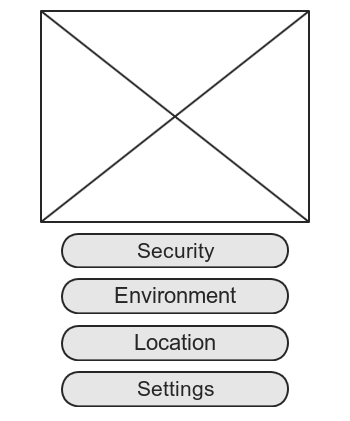
\includegraphics[scale=0.5]{mock_home}
    \caption[Wireframe of the home screen]
            {Wireframe of the home screen}
    \label{fig:wireframe-home}
\end{figure}

\begin{figure}[H]
    \centering
    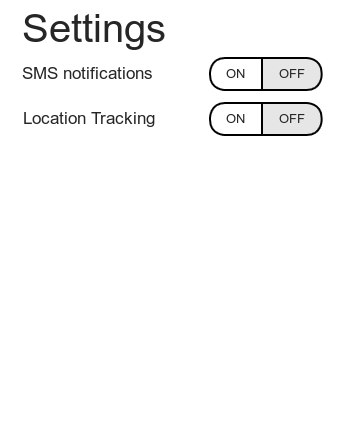
\includegraphics[scale=0.5]{mock_settings}
    \caption[Wireframe of the settings screen]
            {Wireframe of the settings screen}
    \label{fig:wireframe-settings}
\end{figure}

Various portions of the security system can be controlled through the wireframe
in Figure~\ref{fig:wireframe-security}. The entire system can be armed and
disarmed, locks on doors activated and deactivated, and the status of the
windows can be reported. Pressing on the button for window status will bring up
another more detailed screen that lists individual windows and reports their
status, closed or open. Door locks, if it is supported can be locked or
unlocked from this screen if the lock supports it.


\begin{figure}[H]
    \centering
    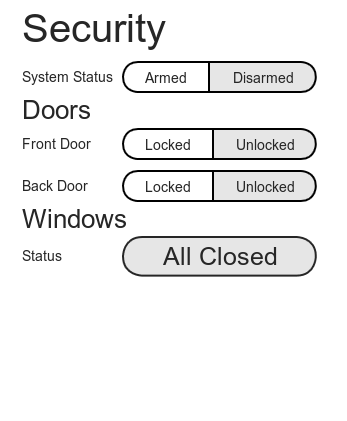
\includegraphics[scale=0.5]{mock_security}
    \caption[Wireframe of the security screen]
            {Wireframe of the security screen}
    \label{fig:wireframe-security}
\end{figure}

Environmental details are controlled in Figure~\ref{fig:wireframe-environment}. The
temperature of the house can be monitored and set. Pressing on the button
labeled "HISTORY" will bring up a graph of the household temperature over a
period of time. This screen can also display images from cameras at the doors
to allow for the user to check who is at the door before unlocking it.
Details from more specific portions of the enviroment can be displayed here as
well. For example, the status of the stove and oven in the kitchen. It is also
possible to report the internal temperature of the oven to ensure that it is
not overheating.

\begin{figure}[H]
    \centering
    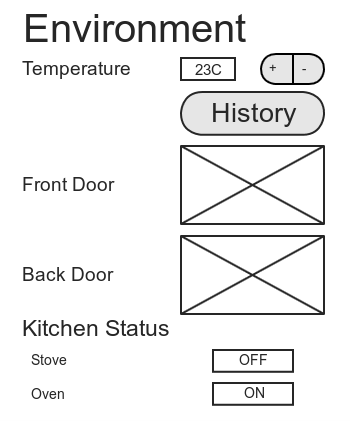
\includegraphics[scale=0.5]{mock_environment}
    \caption[Wireframe of the environment screen]
            {Wireframe of the environment screen}
    \label{fig:wireframe-environment}
\end{figure}

Family member locations -- at least those with smartphones and this
application -- are displayed in Figure~\ref{fig:wireframe-locations}. Each family
member will have a pin on the map to show their location using their device's
GPS capabilities. Clicking on a name will move the map to the present location
of that person. It will also display in text where the family member presently
is located.

\begin{figure}[H]
    \centering
    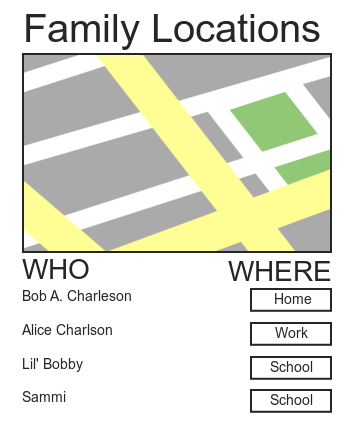
\includegraphics[scale=0.5]{mock_locations}
    \caption[Wireframe of the locations screen]
            {Wireframe of the locations screen}
    \label{fig:wireframe-locations}
\end{figure}



\section{Near-field Communication Keypad}

\section{Web Portal}
\label{sec:web-portal}

\end{document}
